% Density revision 2026-10-04: answers below questions; compact related content.
% ৪.৫ ওয়েবসাইটের কাঠামো
\section{ওয়েবসাইটের কাঠামো (Website Structure)}

% Composition pass 2026-10-04
একটি কলেজের অনেক বিভাগ ও পেজ থাকলে পথ হারিয়ে প্রয়োজনীয় তথ্য খুঁজতে সময় লাগে।

\chFourMotivation{পেজগুলোর সম্পর্ক নির্ধারণ $\rightarrow$ ওয়েবসাইটের কাঠামো $\rightarrow$ ধারাবাহিক, শাখাভিত্তিক বা একাধিক লিংকে সংগঠন $\rightarrow$ ভর্তি ও একাডেমিক তথ্য সহজে পাওয়া।}


\begin{learningbox}
এই অংশ শেষে শিক্ষার্থী পারবে:
\begin{itemize}
\item ওয়েবসাইটের কাঠামোর সংজ্ঞা ও প্রয়োজনীয়তা ব্যাখ্যা করতে।
\item হোমপেজ, প্রধান বিষয়ের পেজ, উপবিষয়ের পেজ ও নেভিগেশনের সম্পর্ক বুঝতে।
\item Linear, Tree, নেটওয়ার্ক/Web-linked ও হাইব্রিড কাঠামো আলাদা করতে।
\item কোন ধরনের ওয়েবসাইটের জন্য কোন কাঠামো বেশি উপযোগী তা নির্ণয় করতে।
\item পরীক্ষার আদলে প্রশ্নে চিত্র ও যুক্তিসহ উত্তর লিখতে।
\end{itemize}
\end{learningbox}

\subsection{ভূমিকা}
ওয়েবসাইটের পেজগুলো যুক্ত করার পরিকল্পনা থাকলে ব্যবহারকারী সহজে প্রয়োজনীয় তথ্যে পৌঁছান। Home, About, Notice, Admission, Result ও Contact পেজের মধ্যে কোন পথে যাওয়া যাবে, তা এই পরিকল্পনায় নির্ধারিত হয়। পেজ দেখতে সুন্দর হলেও সংযোগ দুর্বল হলে তথ্য খুঁজে পাওয়া কঠিন হয়।

\subsection{ওয়েবসাইটের কাঠামো কী?}

\begin{definitionbox}{ওয়েবসাইটের কাঠামো (Website Structure)}
ওয়েবসাইটের পেজ ও তথ্যের পারস্পরিক সম্পর্ক এবং পেজগুলোর সংযোগের বিন্যাসকে ওয়েবসাইটের কাঠামো বলে। মেনু ও লিংক এই সম্পর্ক অনুযায়ী সাজানো হয়।
\end{definitionbox}



\begin{examplebox}{সহজ উদাহরণ}
একটি কলেজ ওয়েবসাইটে Home পেজ থেকে About, Notice, Result ও Contact পেজে যাওয়া যায়। আবার Notice পেজ থেকে Result পেজের লিংক থাকতে পারে। এই পেজগুলোর সম্পর্ক ও লিংক বিন্যাসই ওয়েবসাইটের কাঠামো।
\end{examplebox}

\subsection{ওয়েবসাইটের কাঠামো কেন গুরুত্বপূর্ণ?}

একটি ভালো ওয়েবসাইটে দৃশ্যমান নকশার পাশাপাশি তথ্য ও পেজের সঠিক কাঠামো দরকার। কারণ ব্যবহারকারী মূলত তথ্য খুঁজতে ওয়েবসাইট ব্যবহার করে।

\par\noindent
\begin{minipage}[t]{.48\linewidth}\vspace{0pt}
\begin{itemize}
\item ব্যবহারকারী সহজে তথ্য খুঁজে পায়।
\item পেজগুলোর মধ্যে সম্পর্ক বোঝা সহজ হয়।
\item মেনু ও নেভিগেশন সুন্দরভাবে তৈরি করা যায়।
\item ওয়েবসাইট রক্ষণাবেক্ষণ ও হালনাগাদ করা সহজ হয়।
\end{itemize}
\end{minipage}\hfill
\begin{minipage}[t]{.48\linewidth}\vspace{0pt}
\begin{itemize}
\item নতুন পেজ যুক্ত করা সহজ হয়।
\item শিক্ষা প্রতিষ্ঠান, ব্যবসায়িক ওয়েবসাইট, সংবাদ পোর্টাল বা প্রতিষ্ঠানের ওয়েবসাইট ভালোভাবে সাজানো যায়।
\item সার্চ ইঞ্জিন ওয়েবসাইটের পেজ বুঝতে ও সূচিতে রাখতে সুবিধা পায়।
\item ব্যবহারকারীর অভিজ্ঞতা ভালো হয়।
\end{itemize}
\end{minipage}\par


\Needspace{6\baselineskip}
\subsection{ওয়েবসাইটের কাঠামোর প্রধান উপাদান}

\begin{multicols}{2}
\noindent\begin{minipage}[t]{\linewidth}\vspace{0pt}
\subsubsection{হোমপেজ (Home Page)}

হোমপেজ হলো ওয়েবসাইটের প্রধান প্রবেশপথ। সাইটের মূল ঠিকানা খুললে সাধারণত এটি আগে দেখা যায়; অন্য পেজের সরাসরি লিংক খুললে সেই পেজ আগে আসতে পারে। হোমপেজে গুরুত্বপূর্ণ পেজগুলোর লিংক থাকে।
\end{minipage}\par\smallskip
\noindent\begin{minipage}[t]{\linewidth}\vspace{0pt}
\subsubsection{প্রধান বিষয়ের পেজ (Main Section Page)}

ওয়েবসাইটের বড় বড় বিভাগ বা বিষয়ভিত্তিক পেজকে প্রধান বিষয়ের পেজ বলা যায়। যেমন: Academic, Admission, Notice, Result, Contact।
\end{minipage}\par\smallskip
\noindent\begin{minipage}[t]{\linewidth}\vspace{0pt}
\subsubsection{উপবিষয়ের পেজ (Subsection Page)}

প্রধান বিষয়ের অধীনে থাকা ছোট পেজ হলো উপবিষয়ের পেজ। যেমন: Academic অংশের অধীনে Science, Business Studies ও Humanities পেজ থাকতে পারে।
\end{minipage}\par\smallskip
\noindent\begin{minipage}[t]{\linewidth}\vspace{0pt}
\subsubsection{নেভিগেশন (Navigation)}

নেভিগেশন হলো পেজগুলোর মধ্যে চলাচলের ব্যবস্থা। মেনু বার, ড্রপডাউন মেনু, ফুটার লিংক, ব্রেডক্রাম্ব, অনুসন্ধানের ঘর, Previous/Next বোতাম এবং অভ্যন্তরীণ হাইপারলিংক—এসব নেভিগেশনের অংশ।
\end{minipage}\par\smallskip
\end{multicols}

\begin{center}
\fbox{\parbox{0.92\textwidth}{
\centering
\textbf{উদাহরণ: কলেজের ওয়েবসাইটে পেজগুলোর সম্পর্ক}\\[6pt]
\scaletikz{\begin{tikzpicture}[
  node distance=1.15cm and 1.2cm,
  page/.style={draw, rounded corners=2pt, fill=blue!8, minimum width=2.4cm, minimum height=0.72cm, align=center},
  subpage/.style={draw, rounded corners=2pt, fill=green!8, minimum width=2.2cm, minimum height=0.68cm, align=center},
  every path/.style={-latex}
]
\node[page] (home) {Home};
\node[page, below left=of home] (about) {About};
\node[page, below=of home] (notice) {Notice};
\node[page, below right=of home] (contact) {Contact};
\node[subpage, below=of notice] (result) {Result};
\node[subpage, below=of about] (academic) {Academic};
\draw (home) -- (about);
\draw (home) -- (notice);
\draw (home) -- (contact);
\draw (notice) -- (result);
\draw (about) -- (academic);
\draw[dashed, <->] (notice) -- (contact);
\end{tikzpicture}}\\[4pt]
Home পেজ থেকে প্রধান পেজগুলোতে লিংক থাকে; কিছু পেজ আবার সংশ্লিষ্ট পেজের সাথে যুক্ত থাকতে পারে।
}}
\end{center}

\subsection{ওয়েবসাইটের কাঠামোর প্রকারভেদ}

HSC ICT-এর জন্য চার ধরনের ওয়েবসাইটের কাঠামো সবচেয়ে গুরুত্বপূর্ণ:

\begin{enumerate}
\item Linear বা Sequential কাঠামো
\item Tree বা Hierarchical কাঠামো
\item নেটওয়ার্ক বা Web-linked কাঠামো
\item হাইব্রিড কাঠামো
\end{enumerate}

\subsection{লিনিয়ার বা ধারাবাহিক কাঠামো (Linear/Sequential Structure)}

\subsubsection{লিনিয়ার কাঠামো কী?}

\begin{definitionbox}{লিনিয়ার কাঠামো (Linear Structure)}
যে কাঠামোতে ওয়েবপেজগুলো নির্দিষ্ট ক্রমে একটির পর একটি যুক্ত থাকে, তাকে লিনিয়ার বা ধারাবাহিক কাঠামো বলে। ব্যবহারকারী সেই ক্রমে পেজগুলো দেখেন।
\end{definitionbox}

\begin{center}
\fbox{\parbox{0.90\textwidth}{
\centering
\textbf{লিনিয়ার কাঠামোর চিত্র}\\[6pt]
\scaletikz{\begin{tikzpicture}[
  node distance=0.75cm,
  page/.style={draw, rounded corners=2pt, fill=orange!10, minimum width=1.85cm, minimum height=0.68cm, align=center},
  every path/.style={-latex}
]
\node[page] (start) {Start};
\node[page, right=of start] (p1) {Page 1};
\node[page, right=of p1] (p2) {Page 2};
\node[page, right=of p2] (end) {End};
\draw (start) -- (p1);
\draw (p1) -- (p2);
\draw (p2) -- (end);
\end{tikzpicture}}\\[4pt]
যেমন: Instruction $\rightarrow$ Question 1 $\rightarrow$ Question 2 $\rightarrow$ জমা $\rightarrow$ Result
}}
\end{center}

% Related compact discussions; source reading order is retained.
\par\noindent
\begin{minipage}[t]{.48\linewidth}\vspace{0pt}
\subsubsection{বৈশিষ্ট্য}

\begin{enumerate}
\item পেজগুলো একটির পর একটি সাজানো থাকে।
\item ব্যবহারকারী সাধারণত Next বা Previous লিংক ব্যবহার করে।
\item ধারাবাহিক কাজের মূল পথ নির্দিষ্ট থাকে; প্রয়োজনে Previous লিংক দিয়ে আগের ধাপে ফেরা যায়।
\end{enumerate}
\end{minipage}\hfill
\begin{minipage}[t]{.48\linewidth}\vspace{0pt}
\subsubsection{ব্যবহার}

\begin{enumerate}
\item অনলাইন কুইজ
\item ধাপে ধাপে শেখানোর টিউটোরিয়াল
\item অনলাইন কোর্সের পাঠ
\item নিবন্ধন ফর্ম
\item জরিপের ফর্ম
\item পরীক্ষার নির্দেশনার পেজ
\item পণ্য কেনার শেষ ধাপগুলো
\end{enumerate}
\end{minipage}\par\smallskip
\par\noindent
\begin{minipage}[t]{.48\linewidth}\vspace{0pt}
\subsubsection{সুবিধা}
\begin{enumerate}
\item সহজে বোঝা যায়।
\item ধাপে ধাপে শেখার জন্য ভালো।
\item কুইজ বা টিউটোরিয়াল পরিচালনায় কার্যকর।
\item অগ্রগতি পর্যবেক্ষণ করা সহজ।
\end{enumerate}
\end{minipage}\hfill
\begin{minipage}[t]{.48\linewidth}\vspace{0pt}
\subsubsection{অসুবিধা}
\begin{enumerate}
\item মাঝের পেজ বাদ দিয়ে অন্য পেজে যাওয়া কঠিন।
\item বড় ওয়েবসাইটের মূল কাঠামো হিসেবে সবসময় উপযোগী নয়।
\item ব্যবহারকারীর চলাচলের স্বাধীনতা কম থাকে।
\item অনেক পেজ হলে বিরক্তিকর হতে পারে।
\end{enumerate}
\end{minipage}\par

\Needspace{6\baselineskip}
\subsection{ট্রি বা স্তরভিত্তিক কাঠামো (Tree/Hierarchical Structure)}

\subsubsection{ট্রি কাঠামো কী?}

\begin{definitionbox}{ট্রি কাঠামো (Tree Structure)}
যে কাঠামোতে হোমপেজের অধীনে প্রধান বিষয় এবং তার অধীনে উপবিষয়ের পেজ শাখা-প্রশাখার মতো সাজানো থাকে, তাকে ট্রি বা স্তরভিত্তিক কাঠামো বলে।
\end{definitionbox}

\begin{center}
\fbox{\parbox{0.90\textwidth}{
\centering
\textbf{ট্রি কাঠামোর চিত্র}\\[6pt]
\scaletikz{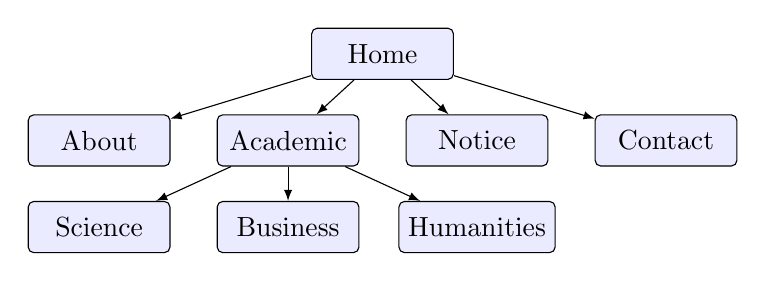
\begin{tikzpicture}[
  level distance=1.1cm,
  sibling distance=2.4cm,
  page/.style={draw, rounded corners=2pt, fill=blue!8, minimum width=1.8cm, minimum height=0.65cm, align=center},
  edge from parent/.style={draw,-latex}
]
\node[page] {Home}
  child { node[page] {About} }
  child { node[page] {Academic}
    child { node[page] {Science} }
    child { node[page] {Business} }
    child { node[page] {Humanities} }
  }
  child { node[page] {Notice} }
  child { node[page] {Contact} };
\end{tikzpicture}}
}}
\end{center}

% Related compact discussions; source reading order is retained.
\par\noindent
\begin{minipage}[t]{.48\linewidth}\vspace{0pt}
\subsubsection{বৈশিষ্ট্য}

\begin{enumerate}
\item একটি মূল বা প্রধান পেজ থাকে।
\item হোমপেজ থেকে বিভাগ ও উপবিভাগ তৈরি হয়।
\item মূল পেজ ও তার অধীন পেজের সম্পর্ক থাকে।
\item নেভিগেশন মেনু, ড্রপডাউন মেনু ও ব্রেডক্রাম্ব ব্যবহার করা যায়।
\end{enumerate}
\end{minipage}\hfill
\begin{minipage}[t]{.48\linewidth}\vspace{0pt}
\subsubsection{ব্যবহার}

\begin{enumerate}
\item স্কুল বা কলেজের ওয়েবসাইট
\item বিশ্ববিদ্যালয়ের ওয়েবসাইট
\item সরকারি ওয়েবসাইট
\item ই-কমার্সের বিষয়ভিত্তিক ওয়েবসাইট
\item গ্রন্থাগারের ওয়েবসাইট
\item প্রতিষ্ঠানের ওয়েবসাইট
\end{enumerate}
\end{minipage}\par\smallskip
\par\noindent
\begin{minipage}[t]{.48\linewidth}\vspace{0pt}
\subsubsection{সুবিধা}
\begin{enumerate}
\item বড় ওয়েবসাইট সহজে সাজানো যায়।
\item বিভাগ ও উপবিভাগ পরিষ্কার বোঝা যায়।
\item মেনু ব্যবস্থা সুন্দর হয়।
\item শিক্ষাপ্রতিষ্ঠান ও অন্যান্য সংস্থার ওয়েবসাইটের জন্য কার্যকর।
\end{enumerate}
\end{minipage}\hfill
\begin{minipage}[t]{.48\linewidth}\vspace{0pt}
\subsubsection{অসুবিধা}
\begin{enumerate}
\item কাঠামো বেশি গভীর হলে ব্যবহারকারী বিভ্রান্ত হতে পারে।
\item অনেক উপবিভাগ হলে নেভিগেশন জটিল হয়।
\item ভুল পরিকল্পনা হলে গুরুত্বপূর্ণ পেজ খুঁজে পাওয়া কঠিন।
\item আগে থেকে ভালো সাইটম্যাপ তৈরি করা দরকার।
\end{enumerate}
\end{minipage}\par

\subsection{নেটওয়ার্ক বা জালিকাবদ্ধ কাঠামো (Network/Web-linked Structure)}

\subsubsection{নেটওয়ার্ক কাঠামো কী?}

\begin{definitionbox}{নেটওয়ার্ক কাঠামো (Network Structure)}
যে কাঠামোতে সম্পর্কিত ওয়েবপেজগুলো বহু লিংকে জালের মতো যুক্ত থাকে, তাকে নেটওয়ার্ক বা জালিকাবদ্ধ কাঠামো বলে। এতে একটি পেজ থেকে একাধিক সংশ্লিষ্ট পেজে সরাসরি যাওয়া যায়।
\end{definitionbox}

\begin{center}
\fbox{\parbox{0.90\textwidth}{
\centering
\textbf{নেটওয়ার্ক কাঠামোর চিত্র}\\[6pt]
\scaletikz{\begin{tikzpicture}[
  node distance=1.6cm and 1.8cm,
  page/.style={draw, rounded corners=2pt, fill=purple!8, minimum width=1.75cm, minimum height=0.66cm, align=center}
]
\node[page] (a) {Page A};
\node[page, right=of a] (b) {Page B};
\node[page, below=of a] (c) {Page C};
\node[page, below=of b] (d) {Page D};
\node[page, right=of d] (e) {Page E};
\draw[<->] (a) -- (b);
\draw[<->] (a) -- (c);
\draw[<->] (b) -- (d);
\draw[<->] (c) -- (d);
\draw[<->] (d) -- (e);
\draw[<->, dashed] (b) -- (e);
\end{tikzpicture}}\\[4pt]
একটি পেজ থেকে একাধিক সংশ্লিষ্ট পেজে যাওয়া যায়।
}}
\end{center}

% Related compact discussions; source reading order is retained.
\par\noindent
\begin{minipage}[t]{.48\linewidth}\vspace{0pt}
\subsubsection{বৈশিষ্ট্য}

\begin{enumerate}
\item পেজগুলোর মধ্যে অনেক লিংক থাকে।
\item ব্যবহারকারী স্বাধীনভাবে বিভিন্ন পেজে যেতে পারে।
\item একটি নির্দিষ্ট পথ থাকে না।
\item সংশ্লিষ্ট বিষয়বস্তু সহজে লিংক করা যায়।
\end{enumerate}
\end{minipage}\hfill
\begin{minipage}[t]{.48\linewidth}\vspace{0pt}
\subsubsection{ব্যবহার}

\begin{enumerate}
\item বড় তথ্যভিত্তিক ওয়েবসাইট, যেমন উইকির মতো ওয়েবসাইট
\item সংবাদ পোর্টাল
\item ব্লগ ওয়েবসাইট
\item গবেষণা বা নির্দেশিকা প্রকাশের ওয়েবসাইট
\item অনলাইন জ্ঞানভান্ডার
\item বড় তথ্য পোর্টাল
\end{enumerate}
\end{minipage}\par\smallskip
\par\noindent
\begin{minipage}[t]{.48\linewidth}\vspace{0pt}
\subsubsection{সুবিধা}
\begin{enumerate}
\item সংশ্লিষ্ট পেজে দ্রুত যাওয়া যায়।
\item তথ্যসমৃদ্ধ ওয়েবসাইটের জন্য ভালো।
\item পেজ দেখার সুযোগ নমনীয় হয়।
\item নির্দিষ্ট তথ্য খোঁজা ও সম্পর্কিত পেজ ঘুরে দেখা সহজ হয়।
\end{enumerate}
\end{minipage}\hfill
\begin{minipage}[t]{.48\linewidth}\vspace{0pt}
\subsubsection{অসুবিধা}
\begin{enumerate}
\item অতিরিক্ত লিংক ব্যবহারকারীকে বিভ্রান্ত করতে পারে।
\item পরিকল্পনা না থাকলে ওয়েবসাইট জটিল হয়।
\item অকার্যকর লিংক বেশি হওয়ার ঝুঁকি থাকে।
\item নতুন ব্যবহারকারী কোথা থেকে শুরু করবে বুঝতে পারে না।
\end{enumerate}
\end{minipage}\par

\subsection{হাইব্রিড কাঠামো (Hybrid Structure)}

\subsubsection{হাইব্রিড কাঠামো কী?}

\begin{definitionbox}{হাইব্রিড কাঠামো (Hybrid Structure)}
দুই বা ততোধিক ধরনের কাঠামোর বৈশিষ্ট্য মিলিয়ে তৈরি ওয়েবসাইটের কাঠামোকে হাইব্রিড বা মিশ্র কাঠামো বলে। প্রয়োজন অনুযায়ী লিনিয়ার, ট্রি ও নেটওয়ার্ক কাঠামো একত্রে ব্যবহার করা যায়।
\end{definitionbox}

\begin{center}
\fbox{\parbox{0.90\textwidth}{
\centering
\textbf{হাইব্রিড কাঠামোর চিত্র}\\[6pt]
\resizebox{.72\linewidth}{!}{\begin{tikzpicture}[
  node distance=0.38cm and 1.25cm,
  page/.style={draw, rounded corners=2pt, fill=teal!8, minimum width=2.1cm, minimum height=0.65cm, align=center},
  flowstep/.style={draw, rounded corners=2pt, fill=orange!10, minimum width=1.8cm, minimum height=0.62cm, align=center},
  every path/.style={-latex}
]
\node[page] (home) {Home};
\node[page, below left=of home] (admission) {Admission};
\node[page, below=of home] (academic) {Academic};
\node[page, below right=of home] (notice) {Notice};
\node[flowstep, below=of admission] (s1) {Step 1};
\node[flowstep, below=of s1] (s2) {Step 2};
\node[flowstep, below=of s2] (pay) {Payment};
\node[page, below=of notice] (result) {Result};
\draw (home) -- (admission);
\draw (home) -- (academic);
\draw (home) -- (notice);
\draw (admission) -- (s1);
\draw (s1) -- (s2);
\draw (s2) -- (pay);
\draw (notice) -- (result);
\draw[dashed, <->] (result) -- (academic);
\end{tikzpicture}}\\[4pt]
Home থেকে অংশগুলো ট্রি আকারে; Admission অংশ লিনিয়ার; Notice/Result সংশ্লিষ্ট লিংকে যুক্ত।
}}
\end{center}

% Related compact discussions; source reading order is retained.
\par\noindent
\begin{minipage}[t]{.48\linewidth}\vspace{0pt}
\subsubsection{বৈশিষ্ট্য}

\begin{enumerate}
\item প্রয়োজন অনুযায়ী একাধিক কাঠামো মিলিয়ে বাস্তব ওয়েবসাইটে ব্যবহার করা যায়।
\item Home পেজ থেকে বিভাগভিত্তিক পেজে যাওয়ার লিংক থাকে।
\item কিছু পেজ ধারাবাহিক ক্রম অনুসরণ করে।
\item কিছু পেজ পরস্পরের সাথে হাইপারলিংক দিয়ে যুক্ত থাকে।
\end{enumerate}
\end{minipage}\hfill
\begin{minipage}[t]{.48\linewidth}\vspace{0pt}
\subsubsection{ব্যবহার}

\begin{enumerate}
\item কলেজ ওয়েবসাইট
\item ই-কমার্স ওয়েবসাইট
\item শেখার প্ল্যাটফর্ম
\item সংবাদ পোর্টাল
\item সরকারি পোর্টাল
\item অনলাইন ভর্তি ব্যবস্থা
\item বড় প্রতিষ্ঠানের ওয়েবসাইট
\end{enumerate}
\end{minipage}\par\smallskip
\par\noindent
\begin{minipage}[t]{.48\linewidth}\vspace{0pt}
\subsubsection{সুবিধা}
\begin{enumerate}
\item বিভিন্ন ধরনের কাজ এক সাইটে থাকলে উপযোগী; ব্যবহারবান্ধব ও নমনীয় বিন্যাস করা যায়।
\item বড় ওয়েবসাইট সুন্দরভাবে সাজানো যায়।
\item ব্যবহারকারী স্বাধীনভাবে পেজ দেখতে পারে।
\item যেখানে দরকার ধারাবাহিক প্রবাহ রাখা যায়।
\end{enumerate}
\end{minipage}\hfill
\begin{minipage}[t]{.48\linewidth}\vspace{0pt}
\subsubsection{অসুবিধা}
\begin{enumerate}
\item নকশার পরিকল্পনা ভালো না হলে জটিল হয়।
\item রক্ষণাবেক্ষণ করতে বেশি দক্ষতা লাগে।
\item পেজের সম্পর্ক ভুল হলে ব্যবহারকারী বিভ্রান্ত হতে পারে।
\item নেভিগেশন ব্যবস্থা ভালোভাবে না করলে ওয়েবসাইট অগোছালো লাগে।
\end{enumerate}
\end{minipage}\par

\subsection{চার ধরনের কাঠামোর তুলনা}

\begin{center}
\begin{tabular}{|p{0.15\textwidth}|p{0.23\textwidth}|p{0.23\textwidth}|p{0.23\textwidth}|}
\hline
\textbf{কাঠামো} & \textbf{বিন্যাস} & \textbf{উপযোগী ক্ষেত্র} & \textbf{প্রধান বৈশিষ্ট্য} \\
\hline
Linear & একটির পর একটি পেজ & কুইজ, টিউটোরিয়াল, ফর্ম & নির্দিষ্ট ক্রম থাকে \\
\hline
Tree & Home থেকে শাখা-প্রশাখা & স্কুল, কলেজ, প্রতিষ্ঠান & বিভাগ ও উপবিভাগ থাকে \\
\hline
নেটওয়ার্ক & পেজগুলো বহু লিংকে যুক্ত & সংবাদ, ব্লগ, wiki & স্বাধীনভাবে পেজ দেখার সুযোগ \\
\hline
Hybrid & একাধিক কাঠামো মিলিত & বড় বাস্তব ওয়েবসাইট & ব্যবহারিক ও নমনীয় \\
\hline
\end{tabular}
\end{center}

\subsection{ওয়েবসাইটের কাঠামো ও নেভিগেশন}

ওয়েবসাইটের কাঠামো হলো পেজগুলোর পারস্পরিক সম্পর্কের বিন্যাস; আর নেভিগেশন সেই সম্পর্ক ব্যবহার করে পেজে যাওয়ার দৃশ্যমান উপায়।

\begin{center}
\begin{tabular}{|p{0.32\textwidth}|p{0.56\textwidth}|}
\hline
\textbf{নেভিগেশন উপাদান} & \textbf{কাজ} \\
\hline
মেনু বার & গুরুত্বপূর্ণ পেজের লিংক একসাথে দেখায় \\
\hline
ড্রপডাউন মেনু & বিভাগ ও উপবিভাগ দেখায় \\
\hline
ফুটার লিংক & পেজের শেষে প্রয়োজনীয় লিংক রাখে \\
\hline
ব্রেডক্রাম্ব (Breadcrumb) & ব্যবহারকারী বর্তমানে ওয়েবসাইটের কোন স্তরে আছে বোঝায় \\
\hline
Previous/Next বোতাম & লিনিয়ার প্রবাহে পেজ পরিবর্তন করে \\
\hline
অভ্যন্তরীণ হাইপারলিংক & সংশ্লিষ্ট পেজ বা অংশে নিয়ে যায় \\
\hline
\end{tabular}
\end{center}

\begin{mistakebox}{সাধারণ ভুল}
মেনু আর ওয়েবসাইটের কাঠামো একই জিনিস নয়। মেনু হলো নেভিগেশনের দৃশ্যমান অংশ; কাঠামো হলো পেজগুলোর সামগ্রিক সম্পর্ক।
\end{mistakebox}

\subsection{প্রয়োজন অনুযায়ী কাঠামো নির্বাচন}

চার ধরনের কাঠামোই বুঝতে হবে। ধারাবাহিক কাজের ক্ষেত্রে \textbf{Linear} এবং বিষয়ভিত্তিক পেজ সাজানোর ক্ষেত্রে \textbf{Tree} বিশেষভাবে উপযোগী।

\begin{keypointbox}{পরীক্ষায় গুরুত্বপূর্ণ বিষয়}
কুইজের প্রশ্ন বা টিউটোরিয়ালের ধাপ নির্দিষ্ট ক্রমে দেখাতে হলে লিনিয়ার কাঠামো সুবিধাজনক, কারণ ব্যবহারকারী ধারাবাহিকভাবে এক পেজ থেকে পরের পেজে যায়। কলেজ বা প্রতিষ্ঠানের বিষয়ভিত্তিক তথ্য সাজাতে ট্রি অথবা হাইব্রিড কাঠামো উপযোগী, কারণ এতে Home পেজ থেকে বিভিন্ন অংশ ও উপবিষয় সাজানো যায়।
\end{keypointbox}

% Original scenario reasoning; Dhaka 2025 printed figure checked separately.
\subsubsection{কাজ অনুযায়ী পেজের সংযোগ}
পেজের সংখ্যা দিয়ে কাঠামোর ধরন নির্ধারিত হয় না। কোন পেজ থেকে কোন পেজে সরাসরি যাওয়ার লিংক আছে এবং ব্যবহারকারী কোন কাজটি করবেন—এই দুটি বিষয় কাঠামো নির্বাচনের ভিত্তি।

\begin{multicols}{2}
\noindent\begin{minipage}[t]{\linewidth}\vspace{0pt}
\begin{keypointbox}{ধারাবাহিক কুইজের ক্ষেত্রে}
নির্দিষ্ট ক্রমে প্রশ্ন ১, ২, ৩ দেখাতে চাইলে লিনিয়ার কাঠামো উপযোগী। Next/Previous লিংক পরের বা আগের প্রশ্নে নিয়ে যায়; নির্ধারিত ধাপ বোঝা সহজ হয়। তবে শুধু পেজের এই সংযোগ দিয়ে সময়, নম্বর বা উত্তর যাচাই স্বয়ংক্রিয় হয় না; সেসবের জন্য অতিরিক্ত ব্যবস্থা দরকার।
\end{keypointbox}
\end{minipage}\par
\noindent\begin{minipage}[t]{\linewidth}\vspace{0pt}
\begin{keypointbox}{বিষয় বেছে অনুশীলনের ক্ষেত্রে}
Home থেকে বিষয়, তারপর সেই বিষয়ের প্রশ্নে যেতে হলে ট্রি কাঠামো স্বাভাবিক। ব্যবহারকারী নিজের বিষয় বেছে নিতে পারে। বিষয়ভিত্তিক ট্রির প্রতিটি প্রশ্নমালায় ধারাবাহিক Next/Previous যোগ করলে ট্রি ও লিনিয়ারের সমন্বয়ে হাইব্রিড কাঠামো হয়।
\end{keypointbox}
\end{minipage}\par
\end{multicols}
হোমপেজ থেকে সব পেজে যাওয়ার লিংক থাকলেও পেজগুলোর মধ্যে সরাসরি সংযোগ নাও থাকতে পারে। এমন অবস্থায় হোমপেজে ফেরার লিংক দিয়ে আগে সেখানে ফিরতে হয়, তারপর গন্তব্য পেজে যেতে হয়। সরাসরি আন্তঃপেজ লিংক থাকলে ধাপ কমে, তবে অতিরিক্ত লিংক পেজ জটিলও করতে পারে। কুইজে বিষয় বা কঠিনতার স্তর বাছাই করতে হলে ট্রি কাঠামো কাজে লাগে। শুধু পেজের সংযোগ দিয়ে সময়, নম্বর বা উত্তর যাচাই স্বয়ংক্রিয় হয় না; এসবের জন্য প্রোগ্রাম প্রয়োজন।


% Original applied explanation; see Chapter04/SOURCES.md.
\subsubsection{এক কাজের জন্য এক ধরনের পথ}
কলেজের Home থেকে Academic, তারপর Science পেজে যাওয়ার বিষয়ভিত্তিক পথ ট্রি কাঠামোর উদাহরণ। ভর্তি-আবেদন পূরণ, তথ্য মিলিয়ে দেখা এবং জমা দেওয়ার ধারাবাহিক কাজ সরলরৈখিক পথের উদাহরণ। একই সাইটে এই দুই পথের ব্যবহার থাকলে মিশ্র কাঠামো পাওয়া যায়।

কাঠামো বাছাইয়ের আগে দর্শকের কাজ লিখবে। বিষয় খুঁজতে বিষয়ভিত্তিক শাখা, ধাপে কাজ শেষ করতে ধারাবাহিক পথ এবং সম্পর্কিত বিষয়ে যেতে পারস্পরিক লিংক দরকার। মেনুর নাম দেখে গন্তব্য বুঝতে পারা ক্লিকের সংখ্যা গোনার চেয়ে বেশি কাজে আসে।


\subsection{সংক্ষিপ্ত অনুশীলন}
\begin{enumerate}
\item ওয়েবসাইটের কাঠামো কী?
\item লিনিয়ার, ট্রি, নেটওয়ার্ক ও হাইব্রিড কাঠামোর বৈশিষ্ট্য লেখ।
\item নির্দিষ্ট ক্রমের কুইজ এবং বিষয় বেছে নেওয়া কুইজের জন্য কাঠামো নির্বাচনের কারণ ব্যাখ্যা কর।
\end{enumerate}

\Needspace{10\baselineskip}
\subsection{বহুনির্বাচনি অনুশীলন}

\begin{multicols}{2}
\begin{enumerate}[leftmargin=*,itemsep=5pt]
\item \begin{minipage}[t]{\linewidth}\vspace{0pt}
ওয়েবসাইটের বিভিন্ন পেজ কীভাবে সাজানো থাকবে—একে কী বলে?
\par ক) Web browser
\par খ) Website structure
\par গ) Search engine
\par ঘ) Web protocol\\
\chFourMCQAnswer{খ) Website structure}
\end{minipage}

\item \begin{minipage}[t]{\linewidth}\vspace{0pt}
যে কাঠামোতে পেজগুলো একটির পর একটি ধারাবাহিকভাবে সাজানো থাকে, সেটি কোন কাঠামো?
\par ক) Tree
\par খ) Linear
\par গ) Network
\par ঘ) Hybrid\\
\chFourMCQAnswer{খ) Linear}
\end{minipage}

\item \begin{minipage}[t]{\linewidth}\vspace{0pt}
কলেজ ওয়েবসাইটের জন্য সাধারণত কোন কাঠামো বেশি উপযোগী?
\par ক) Tree
\par খ) Only Linear
\par গ) Only Random
\par ঘ) None\\
\chFourMCQAnswer{ক) Tree}
\end{minipage}

\item \begin{minipage}[t]{\linewidth}\vspace{0pt}
যে কাঠামোতে বিভিন্ন পেজ জালের মতো লিংক দ্বারা সংযুক্ত থাকে, সেটি কোনটি?
\par ক) Linear
\par খ) Tree
\par গ) Network
\par ঘ) Sequential\\
\chFourMCQAnswer{গ) Network}
\end{minipage}

\item \begin{minipage}[t]{\linewidth}\vspace{0pt}
বাস্তব ওয়েবসাইটে একাধিক কাঠামো মিলিয়ে ব্যবহার করলে তাকে কী বলে?
\par ক) Hybrid Structure
\par খ) Empty Structure
\par গ) Static Structure
\par ঘ) Protocol Structure\\
\chFourMCQAnswer{ক) Hybrid Structure}
\end{minipage}
\end{enumerate}
\end{multicols}

\subsection{সৃজনশীল অনুশীলন}

\begin{practicebox}
\textbf{উদ্দীপক:} একটি শিক্ষা প্রতিষ্ঠান তাদের ওয়েবসাইট তৈরি করতে চায়। ওয়েবসাইটে Home, About, Admission, Notice, Result ও Contact পেজ থাকবে। Admission অংশে শিক্ষার্থীকে Step 1, Step 2, Payment এবং Confirmation পেজ ধারাবাহিকভাবে পূরণ করতে হবে। Notice পেজ থেকে Result পেজ এবং Contact পেজে লিংক থাকবে।

\begin{enumerate}
\item ক. ওয়েবসাইটের কাঠামো কী?
\item খ. ট্রি কাঠামো শিক্ষা প্রতিষ্ঠানের ওয়েবসাইটের জন্য উপযোগী কেন?
\item গ. উদ্দীপকে Admission অংশ কোন কাঠামো অনুসরণ করেছে—ব্যাখ্যা কর।
\item ঘ. উদ্দীপকের ওয়েবসাইটটি হাইব্রিড কাঠামো বলা যায় কি? বিশ্লেষণ কর।
\end{enumerate}
\end{practicebox}



\subsection{সাধারণ ভুল}

\par\noindent
\begin{minipage}[t]{.48\linewidth}\vspace{0pt}
\begin{itemize}
\item Linear ও ট্রি কাঠামো গুলিয়ে ফেলা।
\item নেটওয়ার্ক কাঠামোকে কম্পিউটার নেটওয়ার্ক টপোলজি মনে করা।
\item হাইব্রিড কাঠামো বোঝাতে শুধু ``মিশ্র'' লিখে ব্যাখ্যা না দেওয়া।
\item প্রশ্নে কাঠামোর চিত্র চাওয়া হলেও তা না আঁকা।
\end{itemize}
\end{minipage}\hfill
\begin{minipage}[t]{.48\linewidth}\vspace{0pt}
\begin{itemize}
\item ধারাবাহিক কুইজের উদ্দীপকেও কোনো যুক্তি ছাড়া ট্রি কাঠামো নির্বাচন করা।
\item ওয়েবসাইটের কাঠামো ও HTML ডকুমেন্ট কাঠামো এক মনে করা।
\item মেনু ও ওয়েবসাইটের কাঠামোকে একই মনে করা।
\end{itemize}
\end{minipage}\par


